% !TeX spellcheck = de_DE


\newglossaryentry{dataset}
{name={Daten},
	description={Ein Datensatz\index{Daten} (Daten) besteht aus einem oder mehreren Datenpunkten 
		und ist eine zentrale Komponente der meisten KI Anwendungen. Diese Anwendungen 
		verwenden Datensätze zum Trainieren und Validieren von KI-Modellen. Verschiedene 
		mathematische Modelle und formale Sprachen wurden entwickelt um Datensätze 
		zu beschreiben und zu analysieren \cite{silberschatz2019database,abiteboul1995foundations,hoberman2009data,ramakrishnan2002database}.  
		Eines der am weitesten verbreiteten Datenmodelle ist das relationale Modell, das 
		Daten in Tabellen (oder Beziehungen) organisiert \cite{silberschatz2019database}.
		Eine Tabelle besteht aus Zeilen und Spalten:
		\begin{itemize} 
			\item Jede Zeile der Tabelle repräsentiert einen einzelnen Datenpunkt.
			\item Jede Spalte der Tabelle entspricht einem bestimmten Attribut (oder Merkmal) der 
			Datenpunkte. 
		\end{itemize}
		Tabelle \ref{tab:temperature} zeigt beispielsweise einen Datensatz mit Wetterbeobachtungen.
		\begin{table}[ht]
			\centering
			\begin{tabular}{|l|c|c|c|c|c|}
				\hline
				\textbf{FMI Station} & \textbf{Year} & \textbf{Month} & \textbf{Day} & \textbf{Time} & \textbf{Temp. [°C]} \\ 
				\hline
				Kustavi Isokari & 2023 & 4 & 1 & 00:00 & -0.2 \\ \hline
				Kustavi Isokari & 2023 & 4 & 2 & 00:00 & -0.1 \\ \hline
				Kustavi Isokari & 2023 & 4 & 3 & 00:00 & -1.0 \\ \hline
				Kustavi Isokari & 2023 & 4 & 4 & 00:00 & -0.4 \\ \hline
				Kustavi Isokari & 2023 & 4 & 5 & 00:00 & 0.9 \\ \hline
			\end{tabular}
			\caption{Beobachtungen der Wetter-Station nahe der finnischen Gemeinde \emph{Kustavi}.}
			\label{tab:temperature}
		\end{table}
		Im relationalen Modell ist die Reihenfolge der Zeilen irrelevant und für 
		jedes Attribut (Spalte) muss ein Wertebereich definiert sein. Diese Wertebereiche 
		entsprechen dem Merkmalsraum der Datenpunkte. Während das relationale Modell
		ein nützliches Instrument für die Beschreibung und Analyse von KI System bietet, ist 
		es unzureichend für die Dokumentation von vertrauenswürdiger KI. Moderne Ansätze wie
		Datenblätter für Datensätze bieten eine umfassendere Dokumentation, einschließlich Details 
		zum Erfassungsprozess des Datensatzes und zur beabsichtigten Verwendung \cite{DatasheetData2021}.},first={dataset},text={dataset}  
}





\newglossaryentry{classification}
{name={Klassifizierung},
	description={Klassifizierung\index{Klassifizierung} bezeichnet ML Anwendungen die darauf abzielen, 
		Datenpunkte in eine von mehreren vorgegebenen Kategorien oder Klassen einzuordnen.
	},first={Klassifizierung},text={Klassifizierung} 
}

\newglossaryentry{optimism_in_face_of_uncertainty}
{name={Optimismus im Angesicht der Unsicherheit},
	description={
		\index{Optimismus im Angesicht der Unsicherheit}
		ML-Methoden verwenden ein Leistungsmaß $\bar{f}(\weights)$ um Modell-Parameter $\weights$ 
		zu lernen. Allerdings haben sie in der Regel keinen direkten Zugriff auf $\bar{f}(\weights)$, 
		sondern nur auf eine Schätzung (oder Annäherung) $f(\weights)$. Zum Beispiel verwenden herkömmliche 
		ML Methoden einen Trainingsfehler als Schätzung für den erwarteten Verlust. 
		Mit einem probabilistischen Modell lässt sich ein Konfidenzintervall $\big[ l^{(\weights)},  u^{(\weights)} \big]$ für jede Wahl von Modellparametern konstruieren. 
		Eine einfache Konstruktion hierfür ist $l^{(\weights)} \defeq f(\weights) - \sigma/2$, $u^{(\weights)} \defeq f(\weights) + \sigma/2$, 
		wobei $\sigma$ ein Maß für die (erwartete) Abweichung von $f(\weights)$ zu $\bar{f}(\weights)$ ist. 
		Es können auch andere Konstruktionen für dieses Intervall verwendet werden, solange sie sicherstellen, 
		dass mit ausreichend hoher Wahrscheinlichkeit $\bar{f}(\weights) \in \big[ l^{(\weights)},  u^{(\weights)} \big]$ gilt. 
		Als Optimist wählen wir $\weights$ gemäß dem günstigsten – aber dennoch plausiblen – Wert 
		$\tilde{f}(\weights) \defeq l^{(\weights)}$ des Leistungsmaßes. Zwei Beispiele für diese Konstruktion 
	    findet man in der strukturellen Risikominimierung \cite[Kap. 11]{ShalevMLBook} sowie bei Methoden für 
	    die sequentielle Entscheidungsfindung 
	    \cite[Abschnitt 2.2]{Bubeck2012}. 
		\begin{figure}[htbp]
			\begin{center}
				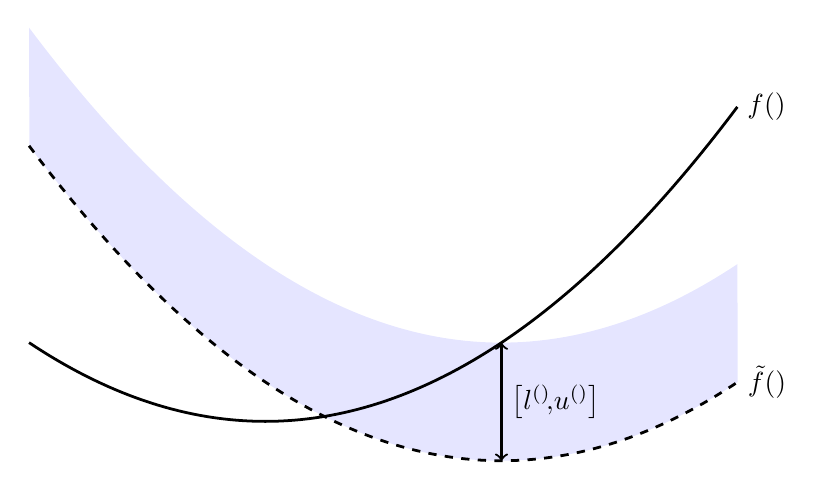
\begin{tikzpicture}[x=3cm, y=1cm]
					% Filled band around the quadratic curve with different boundary curves
					\fill[blue!10] 
					(-1, 5) -- plot[domain=-2:1, samples=100] ({\x+1}, {\x*\x + 1}) -- 
					plot[domain=1:-2, samples=100] ({\x+1}, {\x*\x - 0.5}) -- cycle;
					\node[anchor=west] at (2, 4) {$f(\weights)$};
					\draw[line width=1, domain=-2:1, samples=100,dashed] plot  ({\x+1}, {\x*\x -0.5}) node[right] {$\tilde{f}(\weights)$};
					\draw[line width=1, domain=-1:2, samples=100] plot ({\x}, {\x*\x});
					\draw[<->, thick] (1, -0.5) -- (1, 1) node[midway, right] {$\big[ l^{(\weights)}\!,\!u^{(\weights)} \big]$};
				\end{tikzpicture}
				\caption{Wir verwenden eine Schätzung $f(\weights)$ für das Leistungsmaß $\bar{f}(\weights)$ 
					um ein Konfidenzintervall $\big[ l^{(\weights)},  u^{(\weights)} \big]$ zu konstruieren. Ein Optimist 
					im Angesicht der Unsicherheit wählt Modellparameter $\weights$ gemäß dem günstigsten –
					 aber dennoch plausiblen – Wert $\tilde{f}(\weights) \defeq l^{(\weights)}$.} 
			\end{center}
	\end{figure}},first={Optimismus im Angesicht der Unsicherheit},text={Optimismus im Angesicht der Unsicherheit} 
}